\documentclass[a4paper,12pt]{report}

\usepackage[utf8]{inputenc}
\usepackage{graphicx}
\usepackage{hyperref}
\usepackage[english]{babel}
\usepackage{geometry}
\usepackage{listings}
\usepackage{xcolor}
\usepackage{titlesec}
\usepackage{float}

% Configuration
\geometry{margin=1in}
\hypersetup{
    colorlinks=true,
    linkcolor=blue,
    filecolor=magenta,      
    urlcolor=cyan,
    pdftitle={Beam Audio Flux - Technical Report},
    pdfpagemode=FullScreen,
}

\definecolor{codegreen}{rgb}{0,0.6,0}
\definecolor{codegray}{rgb}{0.5,0.5,0.5}
\definecolor{codepurple}{rgb}{0.58,0,0.82}
\definecolor{backcolour}{rgb}{0.95,0.95,0.92}

\lstdefinestyle{mystyle}{
    backgroundcolor=\color{backcolour},   
    commentstyle=\color{codegreen},
    keywordstyle=\color{magenta},
    numberstyle=\tiny\color{codegray},
    stringstyle=\color{codepurple},
    basicstyle=\ttfamily\footnotesize,
    breakatwhitespace=false,         
    breaklines=true,                 
    captionpos=b,                    
    keepspaces=true,                 
    numbers=left,                    
    numbersep=5pt,                  
    showspaces=false,                
    showstringspaces=false,
    showtabs=false,                  
    tabsize=2
}

\lstset{style=mystyle}

\title{
    \Huge \textbf{Beam Audio Flux} \\
    \large High-Performance Audio Engine \& DAW Prototype \\
    \vspace{0.5cm}
    \textit{Technical Development Report}
}
\author{Beam Development Team}
\date{\today}

\begin{document}

\maketitle

\tableofcontents
\newpage

\chapter{Introduction}

\section{Project Overview}
Beam Audio Flux is a high-performance Digital Audio Workstation (DAW) developed in C++20. Unlike commercial DAWs that rely on heavy frameworks like JUCE or Qt, Beam Audio Flux is built on a "No-Framework" philosophy, utilizing only minimal dependencies: \textbf{SDL3} for hardware abstraction (Windowing, Audio I/O) and \textbf{OpenGL 3.3} for hardware-accelerated rendering.

The primary goal of this project is to create a lightweight, modular, and highly optimized audio environment that bridges the gap between creative "Flux" (node-based modular synthesis) and linear "Splicing" (timeline-based editing).

\section{Core Philosophies}
\begin{itemize}
    \item \textbf{Performance First}: Every subsystem, from the UI rendering to the DSP graph, is designed for cache coherence and minimal allocation.
    \item \textbf{Modern C++}: Leveraging C++20 concepts, smart pointers, and standard algorithms to ensure memory safety without sacrificing speed.
    \item \textbf{Separation of Concerns}: Strict decoupling between the UI (Main Thread) and the Audio Engine (Audio Thread).
\end{itemize}

\chapter{System Architecture}

\section{High-Level Design}
The application is structured into three distinct layers, orchestrated by the \texttt{BeamHost}.

\begin{enumerate}
    \item \textbf{Application Layer (\texttt{BeamHost})}: Manages the OS window, OpenGL context, and the main event loop.
    \item \textbf{Interface Layer (UI)}: A custom component-based UI system that handles user interaction and visualization.
    \item \textbf{Engine Layer (DSP)}: A headless audio processing graph that runs on a high-priority thread.
\end{enumerate}

% \begin{figure}[H]
%     \centering
%     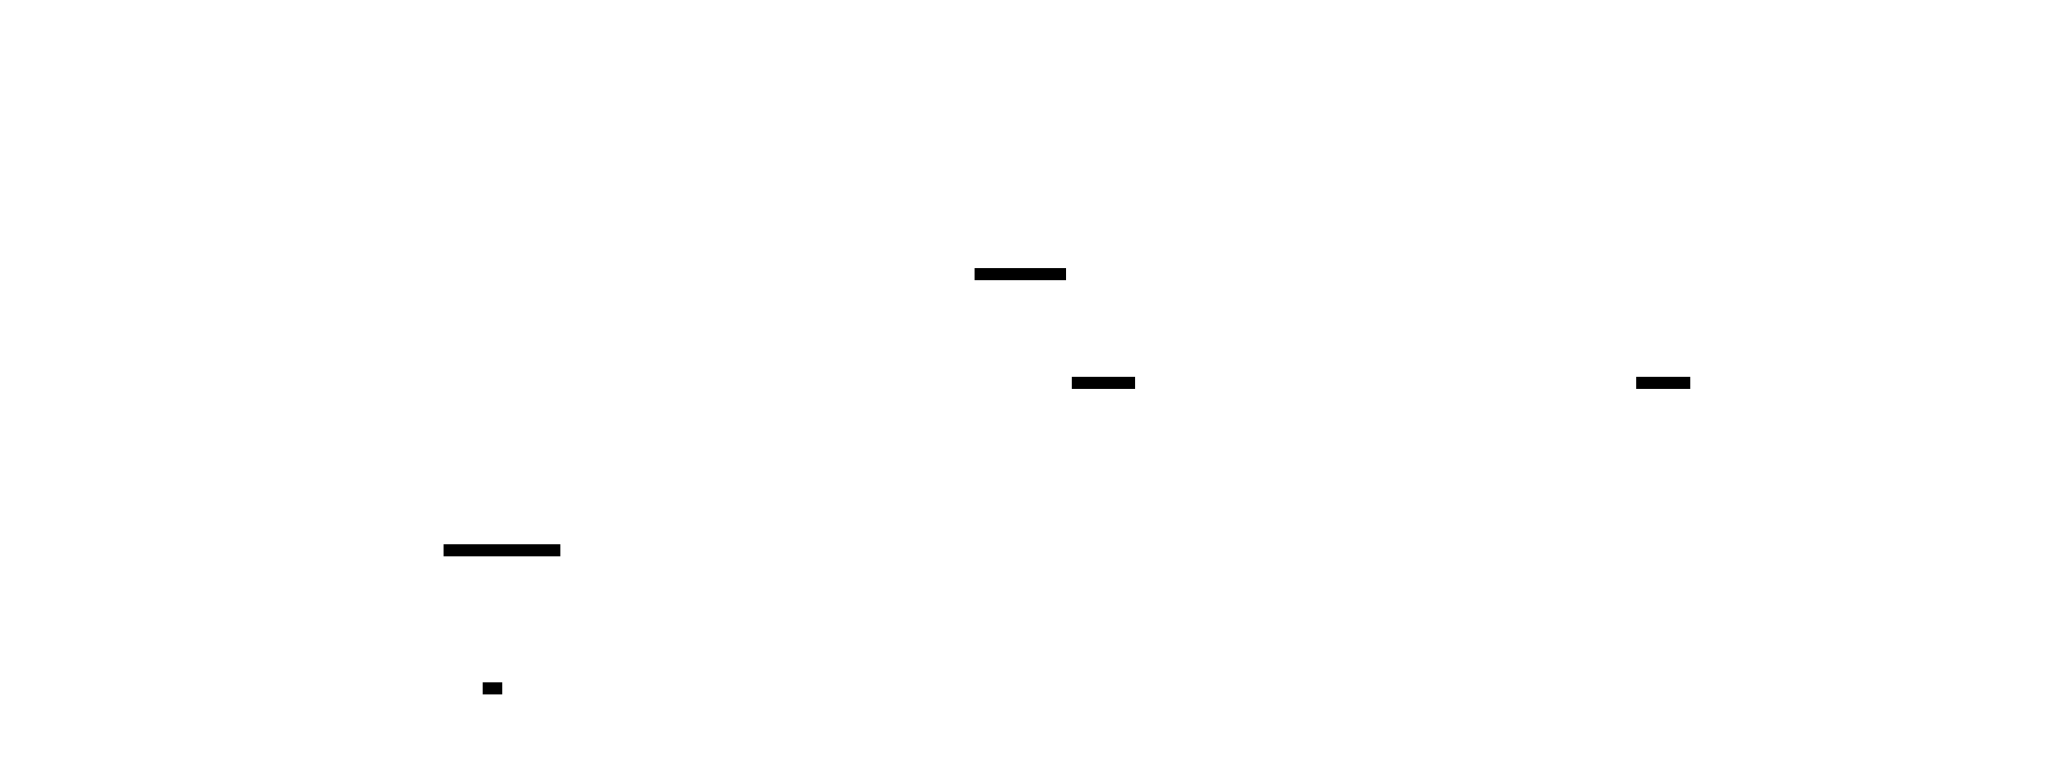
\includegraphics[width=0.9\textwidth]{diagrams/system_overview}
%     \caption{System Overview: The relationship between Host, UI, and Audio Engine.}
%     \label{fig:system_overview}
% \end{figure}

\section{The Application Loop}
The entry point is standard SDL3. The \texttt{BeamHost::run()} method executes a classic game loop:
\begin{lstlisting}[language=C++]
while (isRunning) {
    handleEvents(); // Poll SDL events, pass to InputHandler
    update();       // Update UI logic (animations, state)
    render();       // Batch geometry and submit to GPU
}
\end{lstlisting}

This loop runs independently of the audio callback, ensuring that the UI remains responsive even under heavy DSP load.

\chapter{The Rendering Engine}

To avoid the overhead of immediate-mode GUIs or heavy retained-mode frameworks, Beam Audio Flux implements a custom \textbf{Quad Batcher}.

\section{The \texttt{QuadBatcher}}
In a typical DAW, thousands of small rectangles (knobs, faders, timeline clips) need to be drawn every frame. Issuing a draw call for each would bottleneck the CPU-GPU bus.

The \texttt{QuadBatcher} solves this by:
\begin{enumerate}
    \item \textbf{Accumulation}: UI components submit their geometry (vertices) to a CPU-side buffer.
    \item \textbf{Batching}: The batcher waits until the buffer is full or the frame ends.
    \item \textbf{Single Upload}: It uploads all vertices to the GPU in one go and issues a single \texttt{glDrawElements} call.
\end{enumerate}

\section{UI Components}
The UI is built as a hierarchy of \texttt{Component} objects.
\begin{itemize}
    \item \textbf{Base Class}: \texttt{Component} handles bounds, visibility, and parent-child relationships.
    \item \textbf{Input Handling}: The \texttt{InputHandler} iterates the component tree in Z-order (top-most first) to determine which element consumes a mouse click.
    \item \textbf{Reactive State}: Components like \texttt{Knob} or \texttt{Slider} do not store business logic; they observe parameters and invoke callbacks when changed.
\end{itemize}

\chapter{The Audio Engine (DSP)}

The heart of Beam Audio Flux is the \texttt{FluxGraph}, a dynamic audio processing graph.

% \begin{figure}[H]
%     \centering
%     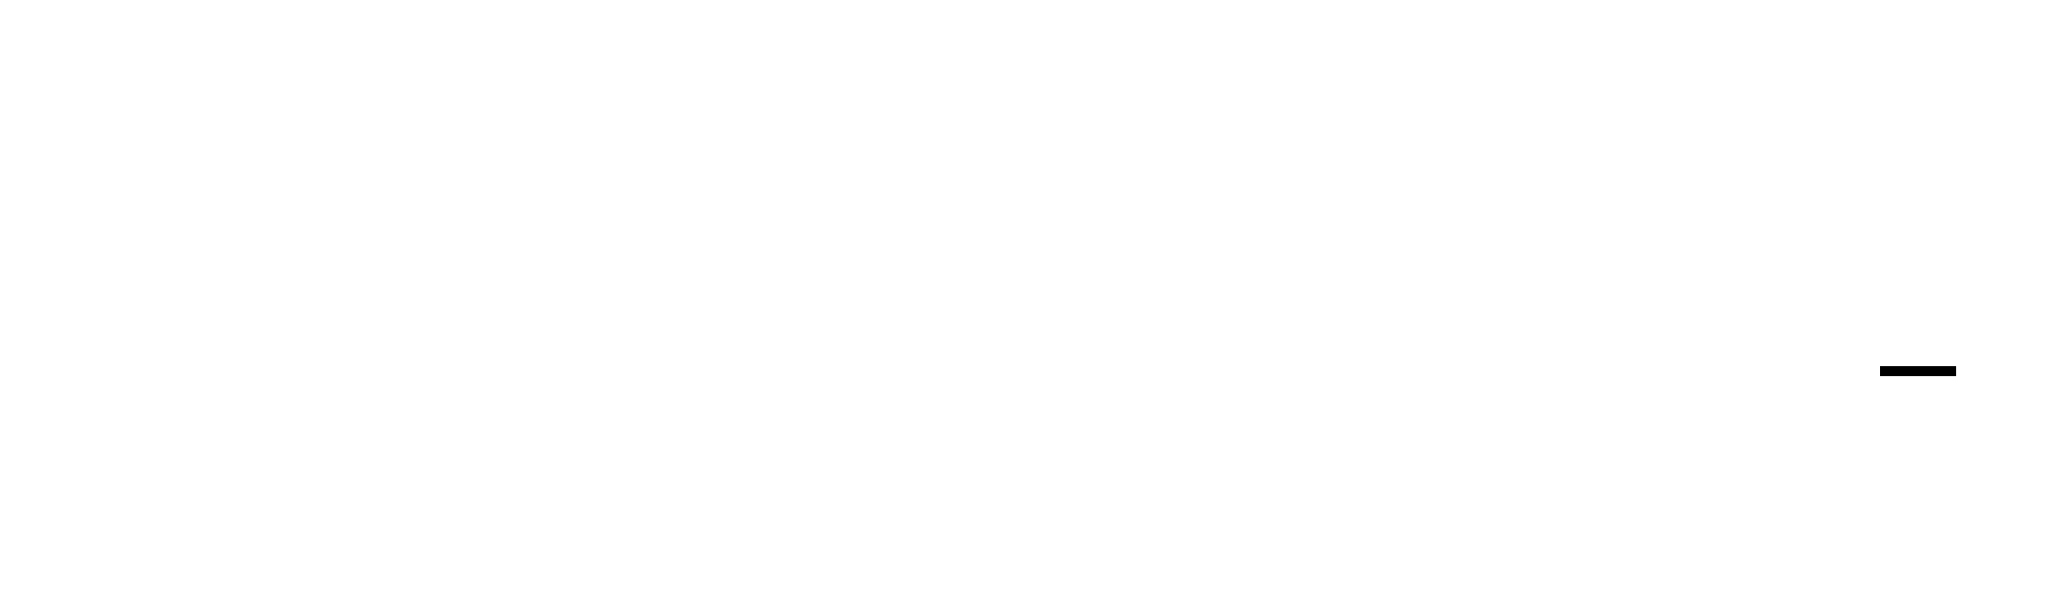
\includegraphics[width=0.9\textwidth]{diagrams/audio_flow}
%     \caption{Audio Data Flow: From Input to Output via the FluxGraph.}
%     \label{fig:audio_flow}
% \end{figure}

\section{Graph Architecture}
Audio processing is modeled as a Directed Acyclic Graph (DAG).
\begin{itemize}
    \item \textbf{Nodes (\texttt{FluxNode})}: Represents a processor (e.g., Filter, Gain, Reverb).
    \item \textbf{Ports}: Each node has N input ports and M output ports.
    \item \textbf{Connections}: Defines the flow of audio buffers between ports.
\end{itemize}

\section{Topological Sorting}
To process the graph, we must ensure that a node is only processed \textit{after} all its dependencies have produced output. We use \textbf{Kahn's Algorithm} to linearize the DAG into a flat "Execution Schedule".

\begin{lstlisting}[language=C++]
// Simplified Logic
void FluxGraph::rebuildSchedule() {
    schedule.clear();
    // 1. Calculate in-degrees for all nodes
    // 2. Queue nodes with 0 in-degree
    // 3. Process queue, appending to schedule and decreasing neighbor degrees
}
\end{lstlisting}

\section{The Process Cycle}
The \texttt{AudioEngine} calls the graph's \texttt{process()} method inside the high-priority SDL audio callback.
\begin{enumerate}
    \item \textbf{Prepare}: Clear all node output buffers.
    \item \textbf{Sum Inputs}: For each node in the schedule, sum the audio from connected upstream ports.
    \item \textbf{Process}: Call \texttt{node->process(context)}.
    \item \textbf{Output}: The result is now available for downstream nodes.
\end{enumerate}

\chapter{Data \& Persistence}

The project state is managed by \texttt{FluxProject} and serialized using \texttt{nlohmann::json}.

\section{Project Structure}
A project file (\texttt{.flux}) contains:
\begin{itemize}
    \item \textbf{Graph Topology}: A list of all nodes, their types, and their unique IDs.
    \item \textbf{Connections}: A list of `(SourceID, Port) -> (DestID, Port)` pairs.
    \item \textbf{Parameters}: The current value of every knob and slider.
    \item \textbf{UI State}: Window positions and layout preferences.
\end{itemize}

\chapter{Conclusion \& Future Work}

Beam Audio Flux has successfully demonstrated that a high-performance DAW can be built with modern C++20 and minimal dependencies. The custom rendering engine provides a fluid 60FPS experience, while the graph-based DSP engine offers the flexibility required for professional audio design.

\section{Roadmap}
\begin{enumerate}
    \item \textbf{Plugin Support}: Wrapper for VST3/CLAP plugins to be hosted as `FluxNode`s.
    \item \textbf{Waveform Splicing}: Advanced time-stretching and slicing tools in the Timeline view.
    \item \textbf{Multi-Threading}: Parallelizing independent graph branches to utilize multi-core CPUs.
\end{enumerate}

\end{document}